\documentclass[10pt]{beamer}
\usetheme{Malmoe}
\usepackage[T2A]{fontenc}
\usepackage[utf8]{inputenc}
\usepackage[english, russian]{babel}
\usepackage{amsmath,pgfplots,booktabs,hyperref,graphicx}
\usepackage[style=verbose-ibid,backend=biber]{biblatex}
\addbibresource{references.bib}

\usepackage{graphicx}
\usepackage{array}
\usepackage{ragged2e}
\let\raggedright=\justifying

\setbeamerfont{title}{size=\LARGE}
\setbeamerfont{frametitle}{size=\large}

\title{Инструменты разделения редких\\ и неравномерно распределённых ресурсов}
\subtitle{25-минутный доклад для экономистов-математиков}
\author{Мещеряков Вадим, Иванова Дарья, Мишаков Андрей, Петрунников Тимур}
\date{\today}

\begin{document}

\maketitle

% ================= СЛАЙД — КРЮЧОК =================
\begin{frame}{Почему это не про «рынок или государство»}
  \begin{columns}
    \column{0.6\textwidth}
    \textbf{Крючок:}
    \begin{itemize}
      \item Население хочет \textbf{тепло}, а не нефть
      \item Спрос на нефть — \textbf{производный}: $D_{oil}(p) = \sum_i a_i D_i(p_i)$,\\
      где $a_i$ — расход нефти на единицу блага $i$
      \item Конкуренция — на уровне \textbf{фирм и государств}, не домохозяйств
    \end{itemize}

    \column{0.4\textwidth}
    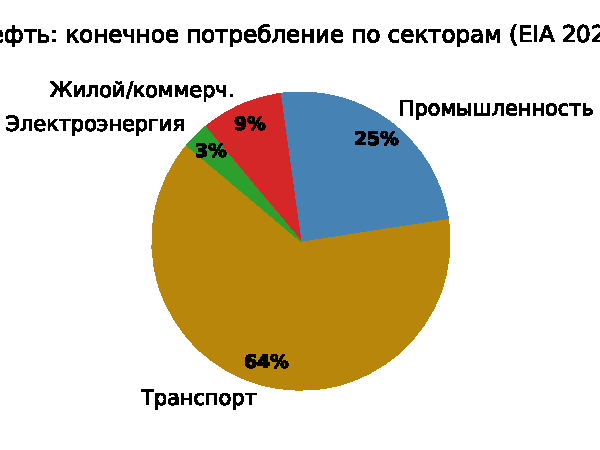
\includegraphics[width=\linewidth]{oil_sector_pie.pdf}
  \end{columns}
  \vspace{0.5cm}
  \begin{alertblock}{}
    «Одна и та же идея — рынок прав — даёт противоположные результаты» (Чили vs Австралия)
  \end{alertblock}
\end{frame}

% ================= СЛАЙД — ТРИ ОСИ =================
\begin{frame}{Три оси — не путать}
  \begin{tabular}{|>{\centering\arraybackslash}p{2.7cm}|>{\centering\arraybackslash}p{2.2cm}|>{\centering\arraybackslash}p{4cm}|} \hline
    \textbf{Ось} & \textbf{Формально} & \textbf{Измеримый индикатор} \\ \hline
    Ограниченность (flow) & $\dot{Q} \le R$ & $R/Q$ (горизонт исчерпания) \\ \hline
    Редкость (scarcity)   & $D(0) > Q$ & $S = D(0)-Q$, эластичность предложения \\ \hline
    Неравномерность       & Концентрация прав & HHI по лицензиям, индекс Джини \\ \hline
  \end{tabular}

  \vspace{0.6cm}
  \begin{exampleblock}{}
    Воздух в чистой местности: $S(0) \le 0$ — \textbf{не редок}, инструменты распределения не нужны.
  \end{exampleblock}
\end{frame}

% ================= СЛАЙД — ИНДИКАТОРЫ РЕДКОСТИ =================
\begin{frame}{Как измерить редкость и неравномерность}
  \begin{columns}[t]
    \column{0.5\textwidth}
    \textbf{Редкость:}
    \[
    \eta = \frac{\Delta Q/Q}{\Delta p/p}
    \]
    $\eta\to 0$ — цена не снимает дефицит.\\
    Нефть: $\eta\approx 0.05$ (коротк.\ период). Органы: $\eta = 0$.

    \column{0.5\textwidth}
    \textbf{Неравномерность:}
    \[
    G = \frac{\sum_{i,j}|x_i-x_j|}{2n^2\mu}, \qquad HHI=\sum_i s_i^2
    \]
    $G<0.3$ — равномерно, $G>0.5$ — остро.\\
    $HHI>1800$ — высокая концентрация (порог DOJ/FTC 2023).
  \end{columns}
\end{frame}

% ================= СЛАЙД — МАТРИЦА =================
\begin{frame}{Матрица исключаемость / соперничество}
  \centering
  \begin{tikzpicture}
    \draw[->, very thick] (0,0) -- (7,0) node[right] {\textit{Исключаемость}};
    \draw[->, very thick] (0,0) -- (0,7) node[above] {\textit{Соперничество}};
    \draw[thick] (0,0) rectangle (3.5,3.5) node[midway] {\textbf{Общественные}};
    \draw[thick] (3.5,0) rectangle (7,3.5) node[midway] {\textbf{Клубные}};
    \draw[thick] (0,3.5) rectangle (3.5,7) node[midway] {\textbf{Commons / откр.\ доступ}};
    \draw[thick] (3.5,3.5) rectangle (7,7) node[midway] {\textbf{Частные}};
  \end{tikzpicture}
\end{frame}

% ================= СЛАЙД — ИНСТРУМЕНТАРИЙ =================
\begin{frame}{Инструментарий — три блока}
  \begin{columns}
    \column{0.3\textwidth}
    \textbf{Собственность}
    \begin{itemize}
      \item Частная (ITQ)
      \item Государственная (концессии)
      \item Commons (Остром)
    \end{itemize}

    \column{0.35\textwidth}
    \textbf{Распределение}
    \begin{itemize}
      \item Аукцион (Vickrey)
      \item Очередь / лотерея
      \item Переуступаемые квоты
    \end{itemize}

    \column{0.27\textwidth}
    \textbf{Ограничение}
    \begin{itemize}
      \item Налог Пигу
      \item Cap-and-trade
      \item Технология / лимит
    \end{itemize}
  \end{columns}
  \vspace{0.4cm}
  \footnotesize 8 принципов Остром: границы, локальные правила, коллективный выбор, мониторинг, градуированные санкции, разрешение конфликтов, признание извне, вложенность.
\end{frame}

% ================= СЛАЙД — ВОДА (ЧИЛИ/АВСТРАЛИЯ) =================
\begin{frame}{Вода: Чили (1981--2022) vs Австралия (Murray--Darling)}
  \begin{columns}
    \column{0.45\textwidth}
    \begin{tabular}{|>{\centering\arraybackslash}p{2.2cm}|>{\centering\arraybackslash}p{2.5cm}|} \hline
      \textbf{Чили} & \textbf{Австралия} \\ \hline
      Частная, отделена от земли & Государственная (entitlement) \\ \hline
      Широкий рынок & Аллокация в рамках cap \\ \hline
      \textbf{Нет жёсткого потолка} & \textbf{Cap} (экология) \\ \hline
      Падение стока (Petorca) & Водопольз.\ $-$33..67\%,\newline GVIAP $-$14..20\% \\ \hline
    \end{tabular}
    \footnotesize \textit{Источники: Bauer (1998), Budds (2008/09), Grafton et al.\ (2014), Kirby et al.\ (2014)}

    \column{0.53\textwidth}
    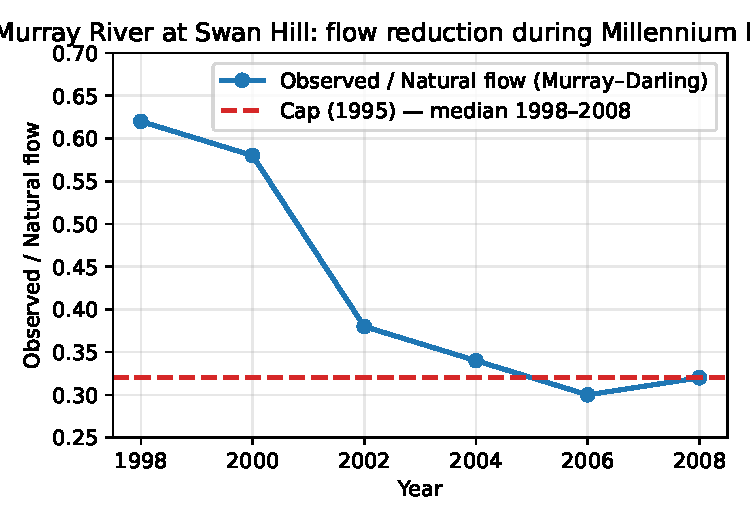
\includegraphics[width=\linewidth]{murray_flow_ratio.pdf}
  \end{columns}
  \vspace{0.2cm}
  \footnotesize С 2022 г.\ в Чили действует реформа (Закон 21.435): права ограничены 30 годами, приоритет — водоснабжение населения.
\end{frame}

% ================= СЛАЙД — ФОРМАЛЬНАЯ СУТЬ =================
\begin{frame}{Формальная суть}
  \begin{columns}
    \column{0.5\textwidth}
    \centering\textbf{Чили — без жёсткого потолка}
    $$q_i \ge 0,\quad \sum q_i \text{ не ограничена}$$
    Цена $\to$ предельные издержки, \textbf{не} экологическая ценность воды.

    \column{0.5\textwidth}
    \centering\textbf{Австралия — внутри Cap}
    $$\bar{Q} = \sum q_i,\quad q_i = e_i \cdot \frac{\bar{Q}}{\sum e_i}$$
    Торговля \textit{долей} потолка. В засуху $\bar{Q}$ падает — цена растёт, \textbf{но объём $\le \bar{Q}$}.
  \end{columns}
  \vspace{0.5cm}
  \begin{alertblock}{}
    Одна и та же конструкция (торгуемые права) $\Rightarrow$ разный результат — в зависимости от наличия жёсткого потолка.
  \end{alertblock}
\end{frame}

% ================= СЛАЙД — ВАЙЦМАН =================
\begin{frame}{Правило Вайцмана (1974): цена vs количество}
  \centering
  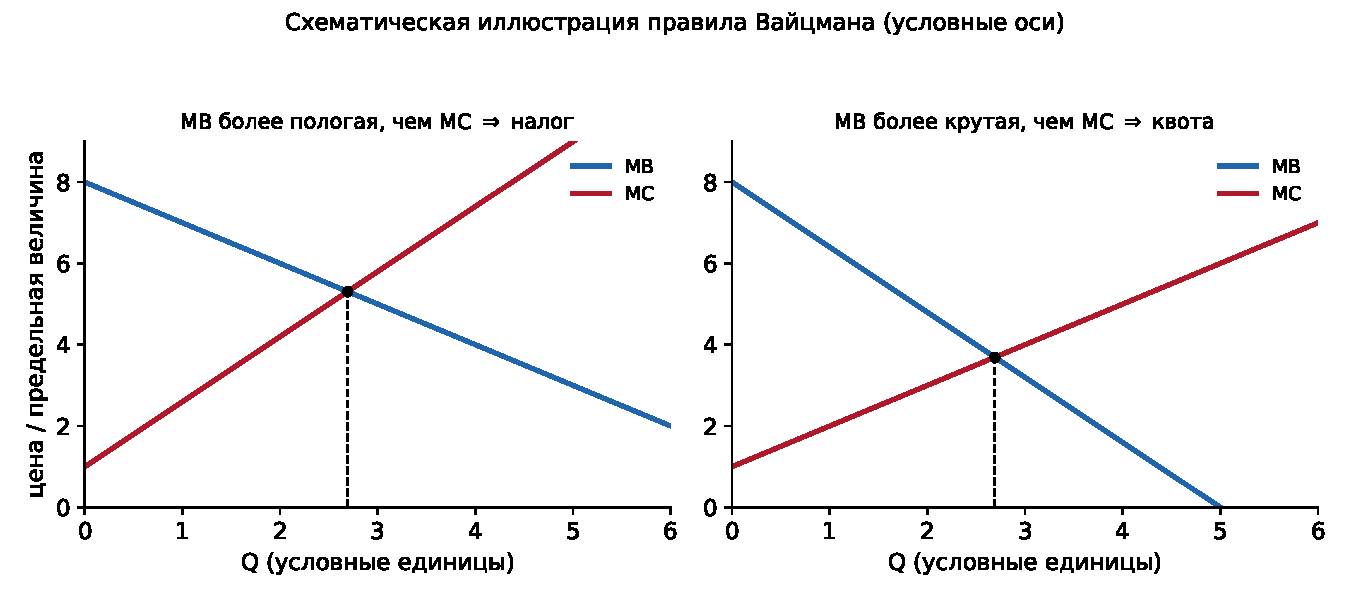
\includegraphics[width=0.85\linewidth]{weitzman_schematic.pdf}
  \vspace{0.3cm}

  \begin{block}{}
    $e < f$ (MB более пологая) $\Rightarrow$ \textbf{налог}; $e > f$ (MB более крутая) $\Rightarrow$ \textbf{квота}. \\
    При риске катастрофы вблизи порога — квота (Weitzman 2009).
  \end{block}
  \footnotesize $\displaystyle \frac{L_{\text{price}}}{L_{\text{quota}}} = \left( \frac{e}{f} \right)^2$ (квадратичные потери, неопределённость в $MC$)
\end{frame}

% ================= СЛАЙД — VCG И ГЕЙЛ-ШЕПЛИ =================
\begin{frame}{Формальные механизмы: VCG и Гейл--Шепли}
  \begin{columns}[t]
    \column{0.5\textwidth}
    \textbf{VCG (правило Кларка):}
    \[
    p_i = \max_{x} \sum_{j\ne i} v_j(x) - \sum_{j\ne i} v_j(x^*)
    \]
    Дорога A--B (стоимость 12): $v_A=8$, $v_B=6$, $v_C=0$.\\
    $p_A=6$, $p_B=4$, $p_C=0$.\\
    Сумма платежей $10<12$ — бюджетный дефицит правила Кларка.

    \column{0.5\textwidth}
    \textbf{Гейл--Шепли:}
    Оба $m_1,m_2$ хотят $w_1$ — конфликт.\\
    $w_1$ выбирает $m_2$ (свой первый выбор), $m_1$ уходит к $w_2$.\\
    Итог: стабильное паросочетание без денег.
  \end{columns}
  \vspace{0.3cm}
  \footnotesize VCG — когда можно оценить выгоды, но нет рынка. Гейл--Шепли — когда деньги запрещены (резидентура, школы, обмен почками).
\end{frame}

% ================= СЛАЙД — DCF / РЕНТА =================
\begin{frame}{Стоимость права: DCF и рента}
  \[
  V_0 = \sum_{t=1}^{T} \frac{q_t(P_t-C_t)}{(1+r)^t}, \qquad
  \text{бессрочно: } V_0 = \frac{R}{r}
  \]
  \begin{itemize}
    \item Рента $1000$/год, 5 лет, $r=5\%$: $V_0\approx 4329.5$ (не 5000 — дисконт).
    \item При стохастическом $TAC_t$ и цене: $\mathrm{Cov}(TAC_t, P_t-C_t)<0$ обычно $\ne 0$ — не разделять матожидания.
    \item Метод Монте-Карло даёт не одно число, а распределение: $V_{5\%}, V_{95\%}$.
  \end{itemize}
  \footnotesize Оговорка: при истощении ресурса рента растёт темпом $r$ (Хотеллинг) — $V_0=R/r$ верно только при примерно постоянной ренте.
\end{frame}

% ================= СЛАЙД — ПЕРКИНС: РЕНТА В РЕАЛЬНОСТИ =================
\begin{frame}{Джон Перкинс: рента $R_t$ в реальности}
  \textbf{Кто контролирует ресурс и куда уходит рента $q_t(P_t-C_t)$?}
  \vspace{0.3cm}

  Капитал как средство доступа к чужому ресурсу:
  \begin{itemize}
    \item Страна берёт крупный кредит под инфраструктуру
    \item Обслуживание долга становится первым требованием к ренте
    \item Кредитор получает экономическое и политическое влияние
  \end{itemize}
  \footnotesize \textit{Confessions of an Economic Hit Man} (2004) — мемуары одного участника, не аудированные данные; далее — иллюстрация тезиса, а не проверенная статистика.
\end{frame}

\begin{frame}{Разбиение ренты по Перкинсу: Эквадор}
  \centering
  \begin{tabular}{|>{\raggedright\arraybackslash}p{6cm}|>{\centering\arraybackslash}p{2.5cm}|}
    \hline
    \textbf{Получатель} & \textbf{Доля от 100\$} \\ \hline
    Нефтяные компании & 75\$ \\ \hline
    Обслуживание внешнего долга & 18.75\$ \\ \hline
    Армия и госаппарат & большая часть остатка \\ \hline
    Здравоохранение, образование, бедность & $\approx$2.5\$ \\ \hline
  \end{tabular}
  \vspace{0.4cm}

  \footnotesize Даже при формально государственной собственности на ресурс почти вся рента уходит держателям институциональных прав.
\end{frame}

\begin{frame}{Судьба Эквадора в 2008--2009 гг.}
  \textbf{Проверяемая часть истории — в отличие от мемуаров.}
  \begin{itemize}
    \item Аудит объявил облигации 2012/2030 (\$3.24 млрд) нелегитимными
    \item Дефолт в ноябре--декабре 2008 г.
    \item Голландский аукцион 2009 г.: выкуп по 35\% от номинала, около 91\% держателей согласились
    \item Выкуп обошёлся в $\approx$\$1.1 млрд; долг снизился с 18.6\% до 14.2\% ВВП
    \item Возврат на рынок облигаций — в 2014 г.
  \end{itemize}
\end{frame}

% ================= СЛАЙД — UNOS =================
\begin{frame}{UNOS: распределение печени — MELD 3.0}
  \begin{columns}
    \column{0.6\textwidth}
    \textbf{Компоненты MELD 3.0:}
    \begin{itemize}
      \item Билирубин, МНО, креатинин (лог, cap 3.0)
      \item Натрий, альбумин
      \item Пол: женщина $+1.33$; исключения HCC
    \end{itemize}
    \textbf{Acuity circles (с 2020 г.):}
    \begin{itemize}
      \item DSA/регионы заменены кругами в морских милях
    \end{itemize}
    \textbf{Continuous distribution:}
    \begin{itemize}
      \item Для печени — проект ещё не завершён (стадия анализа, 2025)
    \end{itemize}
  \end{columns}
  \vspace{0.3cm}
  \begin{alertblock}{}
    Третий полюс: \textbf{приоритизация без денег}. Рынок запрещён институционально (NOTA 1984) — Иран, регулируемый рынок почек с 1988 г., редкое исключение.
  \end{alertblock}
\end{frame}

% ================= СЛАЙД — МОНГОЛИЯ =================
\begin{frame}{Монголия: разрушение работавших commons}
  \begin{itemize}
    \item До 1990 г.\ — коллективные хозяйства (негдэл) с общими правилами выпаса
    \item 1990-е: приватизация скота, земля осталась государственной, старые правила исчезли
    \item Поголовье: $\sim$25 млн (1990) $\to$ $\sim$44 млн (конец 1990-х)
    \item Дзуды 1999--2002: $\sim$11 млн голов; дзуд 2009--2010: $\sim$9.7 млн голов
    \item К 2017--2020 гг.\ поголовье $>$66 млн; 70--88\% пастбищ деградированы
  \end{itemize}
  \footnotesize \textbf{Это не «трагедия общин»} в чистом виде: правила выпаса существовали и работали — их разрушили без замены.
\end{frame}

% ================= СЛАЙД — ЗАМЕНЯЕМОСТЬ =================
\begin{frame}{Заменяемость (backstop)}
  \begin{itemize}
    \item Заменитель по цене $p_b$ ограничивает \textit{рост} цены ресурса (Хотеллинг + backstop), но не обязательно снимает саму редкость
    \item Озоноразрушающие вещества: заменитель появился до катастрофы
    \item Органы: нет технологического backstop \textbf{и} рынок запрещён институционально — две разные причины
  \end{itemize}
  \vspace{0.3cm}
  \footnotesize Связь с Вайцманом здесь — аналогия (крутая предельная выгода вблизи порога $\to$ интуитивно ближе к квоте), а не формальный вывод той же модели.
\end{frame}

% ================= СЛАЙД — СИНТЕЗ =================
\begin{frame}{Синтез}
  \centering
  \begin{tabular}{|>{\centering\arraybackslash}p{2.3cm}|>{\centering\arraybackslash}p{2.1cm}|>{\centering\arraybackslash}p{3.4cm}|} \hline
    \textbf{Ресурс} & \textbf{Инструмент} & \textbf{Почему} \\ \hline
    Вода (Чили) & Рынок & Нет жёсткого потолка \\ \hline
    Вода (Австралия) & Cap + trade & Потолок измерим \\ \hline
    Углерод & Вайцман & MB относительно пологая $\to$ налог \\ \hline
    Органы & UNOS (MELD) & Рынок запрещён институционально \\ \hline
  \end{tabular}

  \vspace{0.8cm}
  \begin{block}{}
    \textbf{Набор инструментов:} собственность $\to$ распределение $\to$ ограничение $\to$ аукцион $\to$ паросочетание $\to$ оценка ренты. \\
    Выбор определяет \textbf{не ресурс}, а измеримость параметров и геометрия кривых.
  \end{block}
\end{frame}

% ================= СЛАЙД — ВОПРОС =================
\begin{frame}{Вопрос залу}
  \begin{columns}
    \column{0.9\textwidth}
    \textbf{Вопрос:} \\
    На каком ресурсе из перечисленных вы бы \textbf{запретили} цену? \\
    (вода, органы, радиочастоты, углерод, земля)
  \end{columns}
\end{frame}

\begin{frame}{Основные источники:}
\footnotesize
\begin{itemize}
\item Bauer (1998) --- Against the Current
\item Budds (2008, 2009) --- Geoforum / Lost in the Long Transition
\item Grafton et al.\ (2014) --- Ambio; Kirby et al.\ (2014) --- Agricultural Water Management
\item Weitzman (1974, 2009) --- RES / REStat
\item Nordhaus (2017) --- PNAS
\item Ostrom (1990); Gale \& Shapley (1962); Vickrey (1961)
\item OPTN/UNOS (2020, 2023, 2025); NOTA (1984)
\item Perkins (2004) --- Confessions of an Economic Hit Man
\item World Bank (2022); FAO (2017)
\end{itemize}
\end{frame}

\end{document}
